\documentclass{beamer}
\usepackage{../../../resources/themes/algolymp-light}

\title{Tehnica Two Pointers}
\subtitle{Sliding Window}
\author{Andrei Mihai Ciobanu}
\institute{Algolymp Summer School}
\date{}
\titlegraphic{
\includegraphics[width=3cm]{../../../resources/algolymp-logo.png}}
\setbeamertemplate{frame footer}{Algolymp Summer School}

% ----------------------------------------------------------------
\begin{document}

\begin{frame}
  \titlepage
\end{frame}

\begin{frame}{Cuprins}
  \tableofcontents[hideallsubsections]
\end{frame}

% ================================================================
\section{Tehnica Two Pointers}

\begin{frame}{Two Pointers \textemdash{} ideea generală}
  Menținem doi indici $l$ și $r$ pe un vector. Niciun indice nu dă \textbf{înapoi}.

  \begin{block}{De ce $O(n)$?}
    Fiecare element e adăugat o singură dată (când $r$ trece prin el)
    și eliminat o singură dată (când $l$ trece prin el) $\Rightarrow$ cel mult $2n$ pași $\Rightarrow O(n)$.
  \end{block}

  \smallskip
  Există două variante în funcție de cum se mișcă pointerii:

  \begin{center}
  \begin{tabular}{lll}
    \toprule
    Variantă & Mișcare & Condiție \\
    \midrule
    Pointeri din capete      & $l \to\qquad\leftarrow r$ & vector \textbf{sortat} \\
    Pointeri în același sens & $l \to\qquad r \to$       & elemente \textbf{pozitive} \\
    \bottomrule
  \end{tabular}
  \end{center}
\end{frame}

% ----------------------------------------------------------------
% Pointeri din capete

\begin{frame}[shrink=15]{Pointeri din capete \textemdash{} exemplu}
  $a = [1,\ 3,\ 5,\ 7,\ 9]$ (sortat), $K = 12$. Pornim cu $l=1$, $r=5$.

  \begin{alertblock}{ÃŽntrebare}
    Dacă $a[l]+a[r] \leq K$ și vectorul e sortat, ce putem spune despre
    perechile $(l,\,l{+}1),\,(l,\,l{+}2),\,\ldots,\,(l,\,r{-}1)$?
  \end{alertblock}

  \begin{center}
  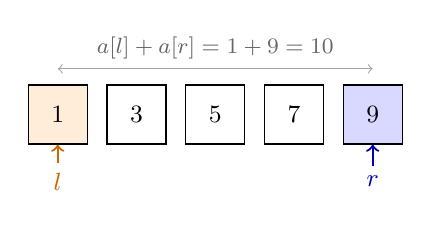
\begin{tikzpicture}[baseline=(current bounding box.center)]
    \node[draw, minimum size=0.75cm, font=\small, fill=orange!15] (box1) at (1,0) {1};
    \node[draw, minimum size=0.75cm, font=\small]                 (box2) at (2,0) {3};
    \node[draw, minimum size=0.75cm, font=\small]                 (box3) at (3,0) {5};
    \node[draw, minimum size=0.75cm, font=\small]                 (box4) at (4,0) {7};
    \node[draw, minimum size=0.75cm, font=\small, fill=blue!15]   (box5) at (5,0) {9};
    \node[orange!80!black, font=\small\bfseries] (lbl) at (1,-0.85) {$l$};
    \draw[->, orange!80!black, thick] (lbl.north) -- (box1.south);
    \node[blue!70!black, font=\small\bfseries]  (rbl) at (5,-0.85) {$r$};
    \draw[->, blue!70!black, thick]  (rbl.north) -- (box5.south);
    \draw[<->, gray!70] (1,0.58) -- (5,0.58)
      node[midway, above, font=\footnotesize, gray!80!black]
        {$a[l]+a[r]=1+9=10$};
  \end{tikzpicture}
  \end{center}

  \begin{center}
  {\footnotesize
  \begin{tabular}{ccccc}
    \toprule
    $l$ & $r$ & $a[l]+a[r]$ & Acțiune & $cnt$ \\
    \midrule
    1 & 5 & $1{+}9=10\leq 12$ & $cnt{+}{=}r{-}l=4$, $l{+}{+}$ & 4 \\
    2 & 5 & $3{+}9=12\leq 12$ & $cnt{+}{=}r{-}l=3$, $l{+}{+}$ & 7 \\
    3 & 5 & $5{+}9=14>12$     & $r{-}{-}$                      & 7 \\
    3 & 4 & $5{+}7=12\leq 12$ & $cnt{+}{=}r{-}l=1$, $l{+}{+}$ & 8 \\
    \bottomrule
  \end{tabular}
  }
  \end{center}

  $l \geq r$ \textemdash{} se oprește. Răspuns: $cnt = 8$.
\end{frame}

\begin{frame}{Numărul de perechi cu suma $\leq K$}
  Sortăm $a$. Menținem $l = 1$ (capăt stâng) și $r = n$ (capăt drept).

  \begin{block}{Cazul $a[l]+a[r] \leq K$ \textemdash{} toate perechile $(l,\,l{+}1),\,\ldots,\,(l,\,r)$ sunt valide}
    Vectorul e sortat: $a[j] \leq a[r]$ pentru orice $j \leq r$, deci
    $a[l]+a[j] \leq a[l]+a[r] \leq K$.
    Adăugăm $r-l$ perechi, avansăm $l$.
  \end{block}

  \begin{block}{Cazul $a[l]+a[r] > K$ \textemdash{} retragem $r$}
    $a[l]$ e cel mai mic element din stânga; dacă suma lui cu $a[r]$
    depășește $K$, nicio pereche cu capăt drept $r$ nu e validă.
  \end{block}

  Ne oprim când $l \geq r$.
\end{frame}

\begin{frame}[fragile]{Implementare \textemdash{} Numărul de perechi cu suma $\leq K$}
  \begin{lstlisting}
sort(a + 1, a + n + 1); // sortam vectorul

int l = 1, r = n;
long long cnt = 0;
while (l < r) {
    if (a[l] + a[r] <= K) {
        cnt += r - l;   // perechile (l, l+1), ..., (l, r)
        l++;
    } else {
        r--;
    }
}
  \end{lstlisting}
\end{frame}

% ----------------------------------------------------------------
% Pointeri in acelasi sens

\begin{frame}[shrink=15]{Pointeri în același sens \textemdash{} exemplu}
  $a = [1,\ 2,\ 3,\ 4,\ 5]$, $K = 9$ \textemdash{} câte secvențe $[l,r]$ au suma $\leq 9$?

  \begin{alertblock}{ÃŽntrebare}
    Dacă $[l, r]$ are suma $\leq K$ (elemente pozitive!), ce putem
    spune despre $[l, l]$, $[l, l{+}1]$, \ldots, $[l, r{-}1]$?
  \end{alertblock}

  \begin{center}
  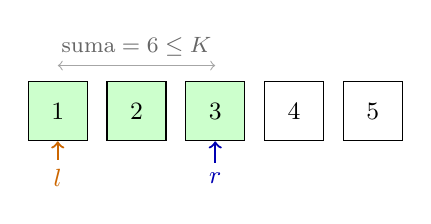
\begin{tikzpicture}[baseline=(current bounding box.center)]
    \node[draw, minimum size=0.75cm, font=\small, fill=green!20] (b1) at (1,0) {1};
    \node[draw, minimum size=0.75cm, font=\small, fill=green!20] (b2) at (2,0) {2};
    \node[draw, minimum size=0.75cm, font=\small, fill=green!20] (b3) at (3,0) {3};
    \node[draw, minimum size=0.75cm, font=\small]                (b4) at (4,0) {4};
    \node[draw, minimum size=0.75cm, font=\small]                (b5) at (5,0) {5};
    \node[orange!80!black, font=\small\bfseries] (lbl) at (1,-0.85) {$l$};
    \draw[->, orange!80!black, thick] (lbl.north) -- (b1.south);
    \node[blue!70!black, font=\small\bfseries]  (rbl) at (3,-0.85) {$r$};
    \draw[->, blue!70!black, thick]  (rbl.north) -- (b3.south);
    \draw[<->, gray!70] (1,0.58) -- (3,0.58)
      node[midway, above, font=\footnotesize, gray!80!black]
        {suma${}=6\leq K$};
  \end{tikzpicture}
  \end{center}

  \begin{center}
  {\footnotesize
  \begin{tabular}{ccccc}
    \toprule
    $l$ & $r$ & suma & Secvențe noi & $ans$ \\
    \midrule
    1 & 3 & 6 & $[1,1],\;[1,2],\;[1,3]$   & 3  \\
    2 & 4 & 9 & $[2,2],\;[2,3],\;[2,4]$   & 6  \\
    3 & 4 & 7 & $[3,3],\;[3,4]$            & 8  \\
    4 & 5 & 9 & $[4,4],\;[4,5]$            & 10 \\
    5 & 5 & 5 & $[5,5]$                    & 11 \\
    \bottomrule
  \end{tabular}
  }
  \end{center}
\end{frame}

\begin{frame}{Numărul de secvențe cu suma $\leq K$}
  \textbf{Problemă:} câte secvențe $[l, r]$ au $a[l] + \ldots + a[r] \leq K$? (elemente pozitive)

  \smallskip
  Extindem $r$ cât putem \textemdash{} fereastra $[l, r]$ e mereu validă (suma $\leq K$).
  Secvențele $[l, l],\, [l, l{+}1],\, \ldots,\, [l, r]$ sunt valide.

  \smallskip
  Adăugăm $r - l + 1$ la contor, apoi eliminăm $a[l]$ și avansăm $l$.
\end{frame}

\begin{frame}[fragile]{Implementare \textemdash{} Numărul de secvențe cu suma $\leq K$}
  \begin{lstlisting}
long long answer = 0, sum = 0;
for (int l = 1, r = 0; l <= n; ++l) {
    // extindem r cat putem
    while (r + 1 <= n && sum + a[r + 1] <= K) {
        sum += a[++r];
    }
    // toate secventele [l, l], [l, l + 1],
    // ..., [l, r] sunt valide
    answer += r - l + 1;
    // eliminam l din secventa
    sum -= a[l];
}
  \end{lstlisting}
\end{frame}

\begin{frame}{Numărul de secvențe cu suma $\geq K$}
  \textbf{Problemă:} câte secvențe $[l, r]$ au $a[l] + \ldots + a[r] \geq K$? (elemente pozitive)

  \smallskip
  Extindem $r$ cât e nevoie \textemdash{} căutăm cel mai mic $r$ pentru care suma $\geq K$.
  Secvențele $[l, r],\, [l, r{+}1],\, \ldots,\, [l, n]$ sunt valide.

  \smallskip
  Adăugăm $n - r + 1$ la contor, apoi eliminăm $a[l]$ și avansăm $l$.

  \smallskip
  \textbf{Observație:} se poate calcula și ca $\dfrac{n(n+1)}{2} - cnt_{< K}$, unde $cnt_{< K}$ = nr.\ secvențe cu suma $< K$.
\end{frame}

\begin{frame}[fragile]{Implementare \textemdash{} Numărul de secvențe cu suma $\geq K$}
  \begin{lstlisting}
long long answer = 0, sum = 0;
for (int l = 1, r = 0; l <= n; ++l) {
    // extindem r cat timp e nevoie
    while (r + 1 <= n && sum < K) {
        sum += a[++r];
    }
    // toate secventele [l, r], [l, r + 1],
    // ..., [l, n] sunt valide
    if (sum >= K) {
        answer += n - r + 1;
    }
    // eliminam l din secventa
    sum -= a[l];
}
  \end{lstlisting}
\end{frame}

% ================================================================
\section{Sliding Window}

\begin{frame}{Fereastră fixă}
  \textbf{Sliding Window}: fereastra are mereu exact $k$ elemente consecutive.

  \begin{block}{Exemplu}
    Suma maximă a $k$ elemente consecutive din $a[1 \ldots n]$.
  \end{block}

  \begin{itemize}
    \item Calculăm suma primei ferestre $[1, k]$
    \item La fiecare pas: adăugăm $a[r]$, scoatem $a[r-k]$
    \item Actualizăm maximul \textemdash{} fără a recalcula de la zero
  \end{itemize}

  \smallskip
  Fiecare element e adăugat și scos o singură dată $\Rightarrow$ $O(n)$.
\end{frame}

\begin{frame}[fragile, shrink]{Implementare \textemdash{} Fereastră fixă}
  \begin{lstlisting}
const int nmax = 100000;
int a[nmax + 1];
int n, k;

long long suma = 0, maxSuma = 0;
for (int i = 1; i <= k; i++) {
    suma += a[i];
}
maxSuma = suma;

for (int r = k + 1; r <= n; r++) {
    suma += a[r] - a[r - k]; // adaugam dreapta, scoatem stanga
    if (suma > maxSuma) {
        maxSuma = suma;
    }
}
  \end{lstlisting}
\end{frame}

% ================================================================
\section{Recapitulare}

\begin{frame}{Recapitulare}
  \begin{center}
  \begin{tabular}{lll}
    \toprule
    Tehnică & Complexitate & Condiție \\
    \midrule
    Pointeri din capete      & $O(n)$ & vector sortat \\
    Pointeri în același sens & $O(n)$ & elemente pozitive \\
    Sliding Window       & $O(n)$ & \textemdash{} \\
    \bottomrule
  \end{tabular}
  \end{center}

  \begin{itemize}
    \item Cheia: nici un indice nu dă înapoi
  \end{itemize}
\end{frame}

\begin{frame}{Probleme de antrenament}
  \begin{enumerate}\footnotesize\itemsep2pt
    \item \href{https://code.algolymp.com/problems/4277}{\textbf{Pair Sum Window Count}}
          \textcolor{gray}{(AlgoCode \#4277)}
    \item \href{https://cses.fi/problemset/task/1640}{\textbf{Sum of Two Values}}
          \textcolor{gray}{(CSES \#1640)}
    \item \href{https://code.algolymp.com/problems/1747}{\textbf{palindrom}}
          \textcolor{gray}{(AlgoCode \#1747 · OJI 2023 VII)}
    \item \href{https://code.algolymp.com/problems/503}{\textbf{secvmin}}
          \textcolor{gray}{(AlgoCode \#503 · ONI 2023 VII)}
  \end{enumerate}
\end{frame}

\begin{frame}{Resurse}
  \begin{enumerate}\itemsep6pt
    \item \href{https://old.algogenius.ro/two-pointers/}{\textbf{AlgoGenius}}
          \textemdash{} Tehnica Two Pointers (RO)
    \item \href{https://usaco.guide/silver/two-pointers?lang=cpp}{\textbf{USACO Guide}}
          \textemdash{} Two Pointers (EN)
    \item \href{https://cdn.sepi.ro/infobits-f1.pdf}{\textbf{Infobits Academy F1}}
          \textemdash{} p. 79 (RO)
  \end{enumerate}
\end{frame}

\end{document}
